\documentclass[12pt]{article}
\usepackage{verbatim}
\usepackage[dvips]{epsfig}
\usepackage{color}
\usepackage{url}
\usepackage[colorlinks=true]{hyperref}

\begin{document}

\section*{GENESIS: Documentation}

{\bf Related Documentation:}
% start: userdocs-tag-replace-items related-do-nothing
% end: userdocs-tag-replace-items related-do-nothing

\section*{De Schutter: Purkinje Cell Model}

\subsection*{Source}

De Schutter E \& Bower JM (1994) An active membrane model of the cerebellar Purkinje cell I. Simulation of current clamp in slice. {\it Journal of Nerurophysiology}. {\bf 71}: 375--400. \\

\noindent De Schutter E \& Bower JM (1994) An active membrane model of the cerebellar Purkinje cell II. Simulation of synaptic responses. {\it Journal of Nerurophysiology}. {\bf 71}: 401--419.

\subsection*{Figures}

\begin{figure}[h]
\centering
   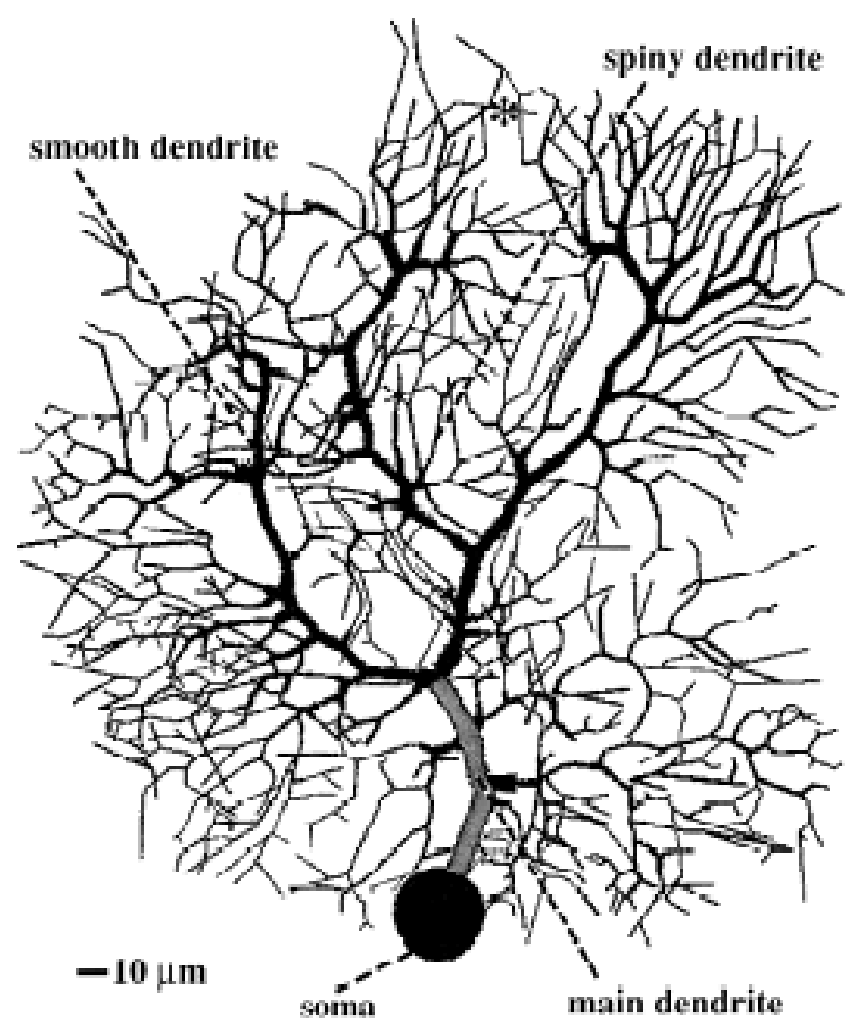
\includegraphics[scale=0.75]{figures/Fig.1.1.eps}
   \caption{Morphology of the Purkinje cell model ({\it cell\,1} of\,\cite{Rapp-P:1994qf}).  The 3 zones with different channel densities (Table 2) are marked
as soma (black), main dendrite (dark gray), and the rest of the dendrites
(black). Dashed lines: recording sites displayed in Figs 3-7. Asterisk: recording
site for Figs. 12 and 13.
electron microscopic (EM)}
   \label{fig:DS1.1}
\end{figure}

\clearpage

\begin{figure}[h]
\centering
   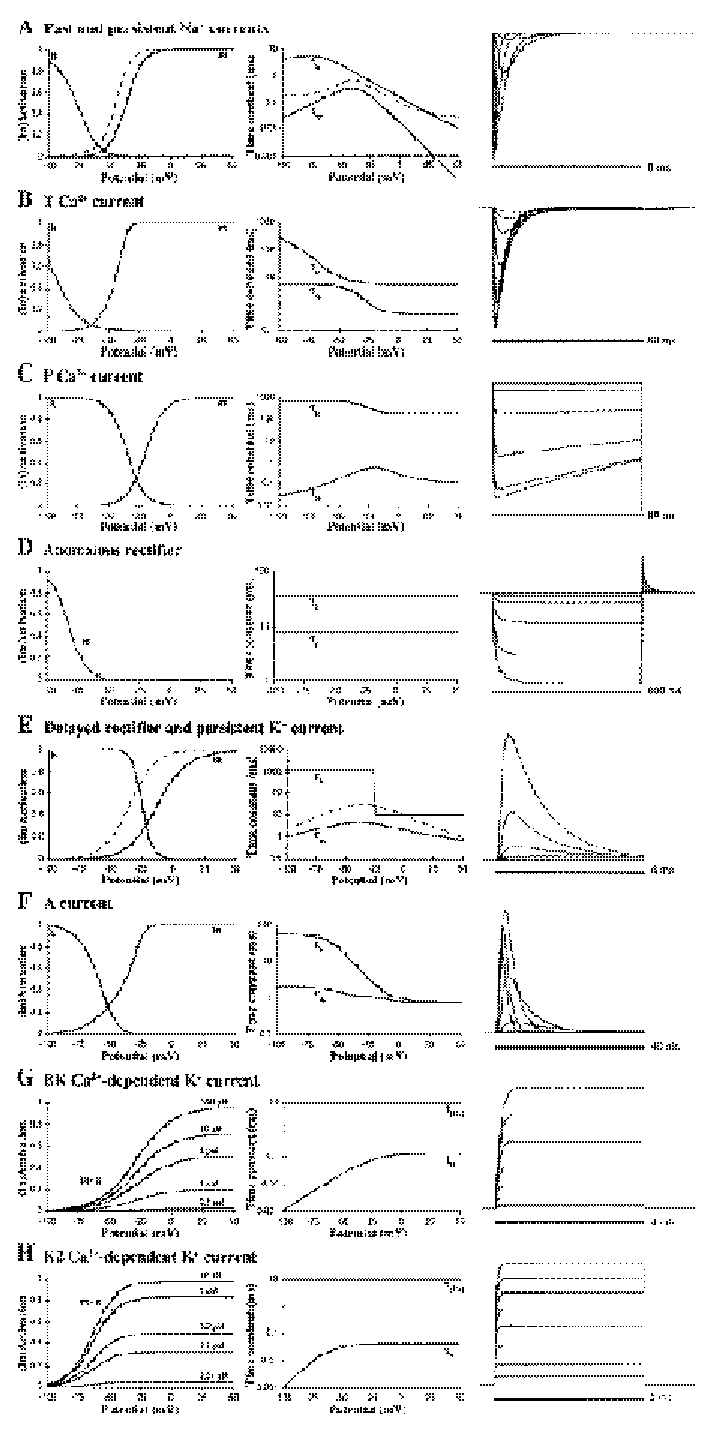
\includegraphics[scale=0.75]{figures/Fig.1.2.eps}
   \caption{Activation and inactivation properties of the ionic conductances in the model. For each conductance steady-state activation and inactivation vs. voltage are plotted at the {\em left}, the time constants of activation ($\tau_m$) and inactivation ($\tau_h$) vs. voltage in the {\em middle} (note the semilogarithmic scale), and a simulation of representative voltage-clamp currents at the {\em right}. $A$ : Fast Na$^+$ current (---) and persistent Na$^+$ current (- - -, no inactivation). The voltage-clamp simulation shows fast sodium (NaF) current only. $B$: T-type Ca$^{2+}$ current. {\it C}: P-type Ca$^{2+}$ current. {\it D}: Anomalous rectifier. Note that this current does not inactivate and that activation is determined by 2 time constants ($\tau_1$ and $\tau_2$\,\cite{Spain-W-J:1987ij}). {\it E}: Delayed rectifier (---) and persistent K+ current (- - - , no inactivation). The voltage-clamp simulation shows Kdr only. {\it F}: A current. {\it G}: High-threshold Ca$^{2+}$-activated K$^+$ current (BK-type). {\it H}: Low-threshold Ca $^{2+}$-activated K$^+$ current (K2-type). Note that for both Ca$^{2+}$-dependent K$^+$ currents activation is controlled by the product of a voltage and a [Ca$^{2+}$]-dependent factor, each with their own time constants ($\tau_V$ and $\tau_{[Ca]}$). The voltage clamps simulate steps from a holding potential of -110 to -70\,mV up to 0\,mV in 10\,mV increments, except for {\it D}, which steps from a holding potential of 0 to -80\,mV up to -10\,mV. The voltage-clamp current amplitude has been scaled arbitrarily because we mainly wanted to demonstrate the current kinetics.}
   \label{fig:DS1.2}
\end{figure}

\clearpage

\begin{figure}[h]
\centering
   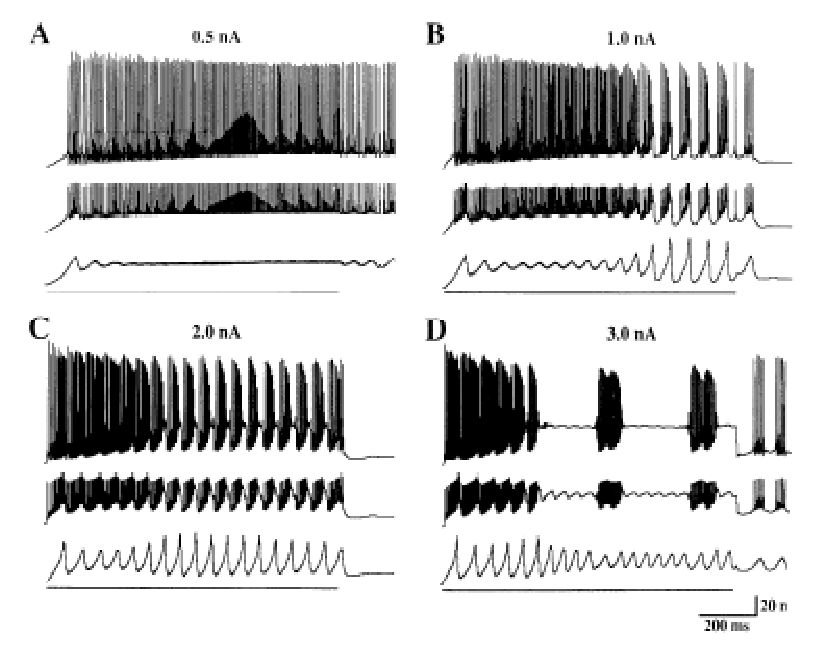
\includegraphics[scale=0.75]{figures/Fig.1.3.eps}
   \caption{Simulation of current injection in the
soma, model PM9. For each current injection amplitude
(A: 0.5\,nA, B: 1.0\,nA, C: 2.0\,nA, D: 3.0\,
nA) 3 recording sites are shown: the soma (top
trace), the main dendrite (middle trace), and a
spiny dendrite (bottom trace). Bar below traces: duration
of current injection.}
   \label{fig:DS1.3}
\end{figure}

\clearpage

\begin{figure}[h]
\centering
   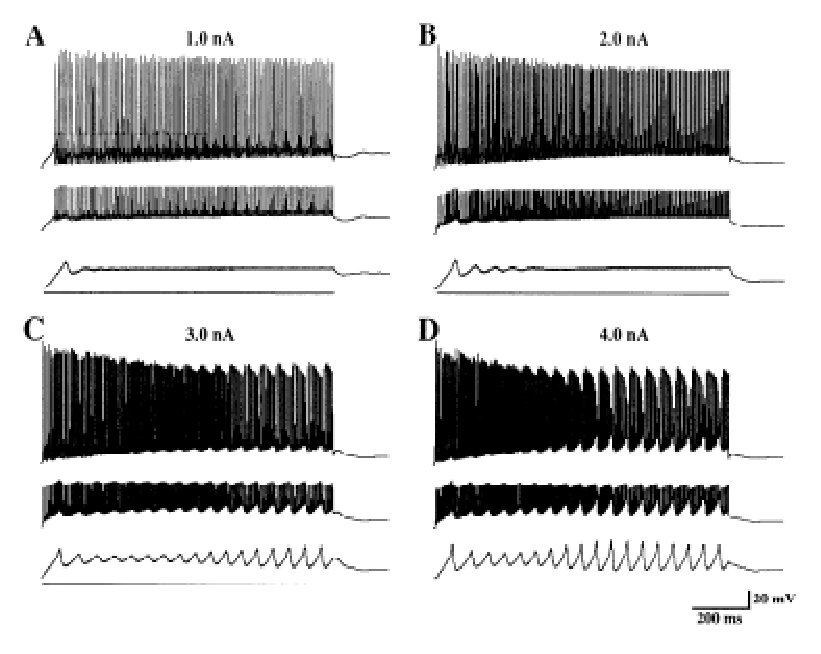
\includegraphics[scale=0.75]{figures/Fig.1.4.eps}
   \caption{Simulation of current injection in the
soma, model PM9. For each current injection amplitude
(A: 0.5\,nA, B: 1.0\,nA, C: 2.0\,nA, D: 3.0\,
nA) 3 recording sites are shown: the soma (top
trace), the main dendrite (middle trace), and a
spiny dendrite (bottom trace). Bar below traces: duration
of current injection.}
   \label{fig:DS1.4}
\end{figure}

\clearpage

\begin{figure}[h]
\centering
   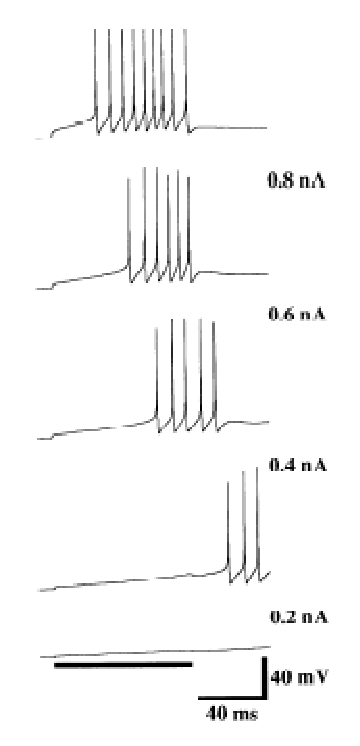
\includegraphics[scale=0.75]{figures/Fig.1.5.eps}
   \caption{Simulation of short current steps just below and above firing threshold in the soma (model PM9). Amplitude of current injection for each trace is indicated. Bar below traces: duration.}
   \label{fig:DS1.5}
\end{figure}

\clearpage

\begin{figure}[h]
\centering
   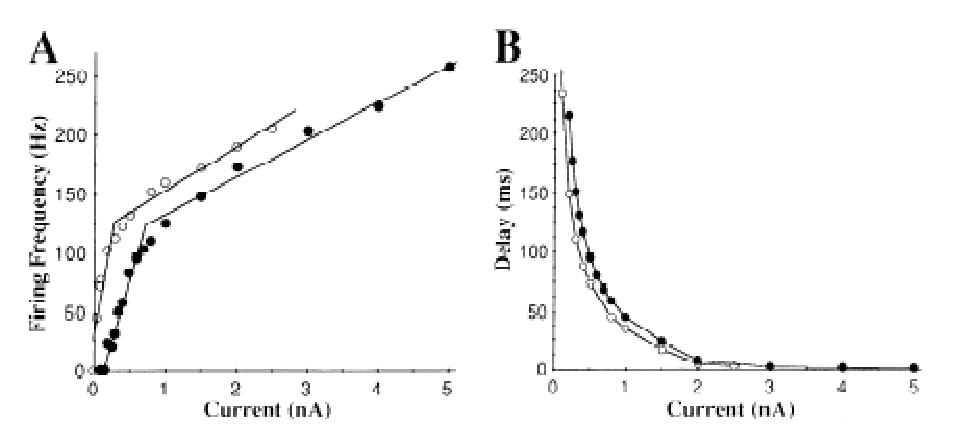
\includegraphics[scale=0.75]{figures/Fig.1.6.eps}
   \caption{Relation of somatic firing response to the amplitude of injected current in models PM9 ($\circ$) and PM10 ($\bullet$). {\it A}: Firing frequency vs. amplitude of injected current [frequency-current ($f$--$I$) curve]. Frequencies were measured in an interval from 300 to 700\,ms after onset of the current injection, before any clear depolarizing spike bursts in the soma. {\it B}: delay between onset of current injection and 1st somatic spike vs. amplitude of injected current.}
   \label{fig:DS1.6}
\end{figure}

\clearpage

\begin{figure}[h]
\centering
   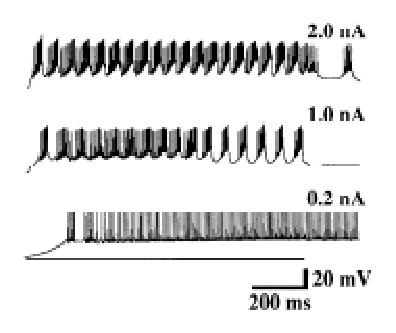
\includegraphics[scale=1]{figures/Fig.1.7.eps}
   \caption{Recordings of membrane potential in the main dendrite in response
to 3 different levels of current injection at the same location, model
PM9. Amplitude of current injection is indicated. Bar below traces: duration.}
   \label{fig:DS1.7}
\end{figure}

\clearpage

\begin{figure}[h]
\centering
   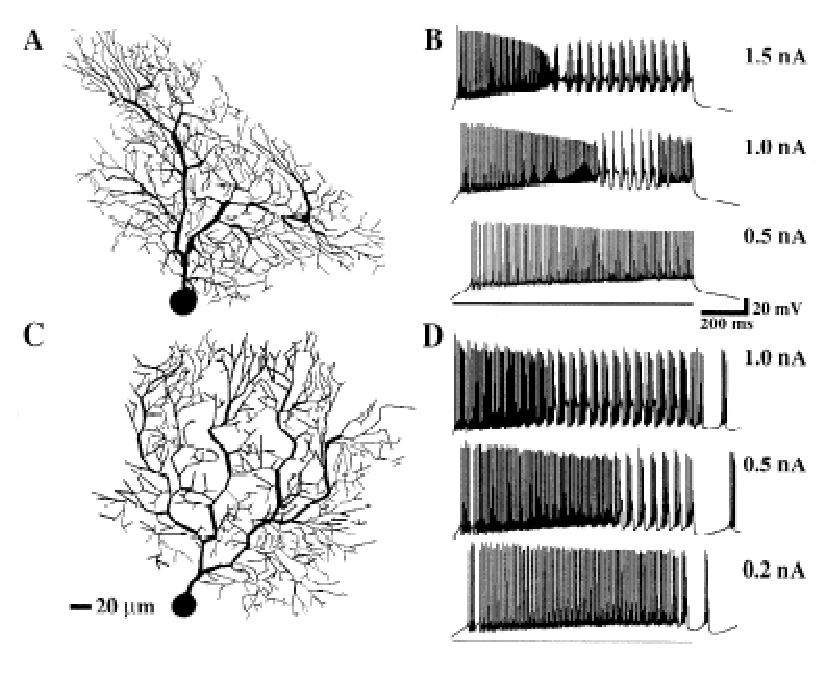
\includegraphics[scale=0.75]{figures/Fig.1.8.eps}
   \caption{Recordings of membrane potential in the main dendrite in response
to 3 different levels of current injection at the same location, model
PM9. Amplitude of current injection is indicated. Bar below traces: duration.}
   \label{fig:DS1.8}
\end{figure}

\clearpage

\begin{figure}[h]
\centering
   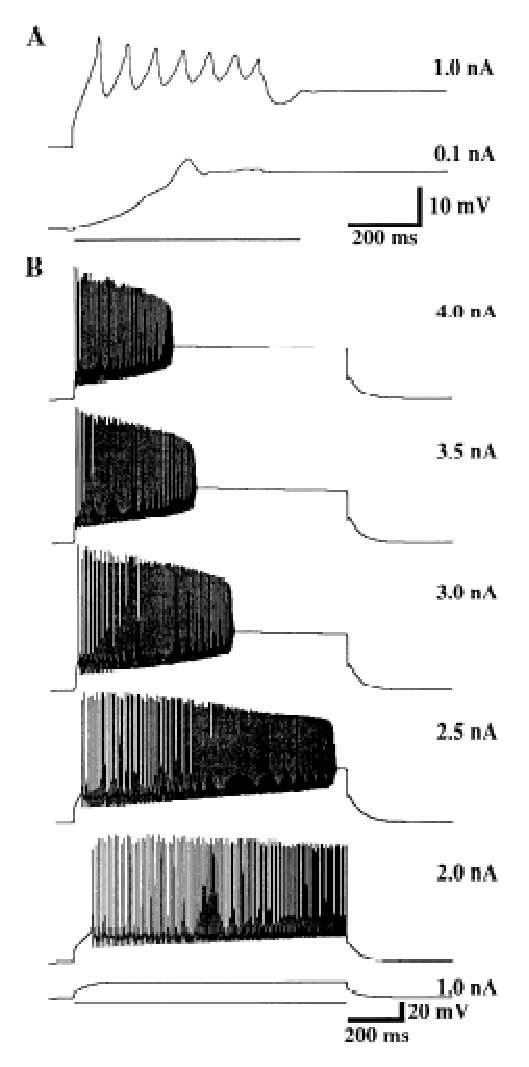
\includegraphics[scale=1]{figures/Fig.1.9.eps}
   \caption{Simulation of channel blocking experiments. {\it A}: Simulation of the effect of blocking Na$^+$ currents by tetrodotoxin (TTX) application. {\it B}: Simulation of the effect of blocking Ca$^{2+}$ currents by Co$^{2+}$ or Cd$^{2+}$ application. Membrane potential in the soma during current injections of indicated amplitudes in the soma.}
   \label{fig:DS1.9}
\end{figure}

\clearpage

\begin{figure}[h]
\centering
   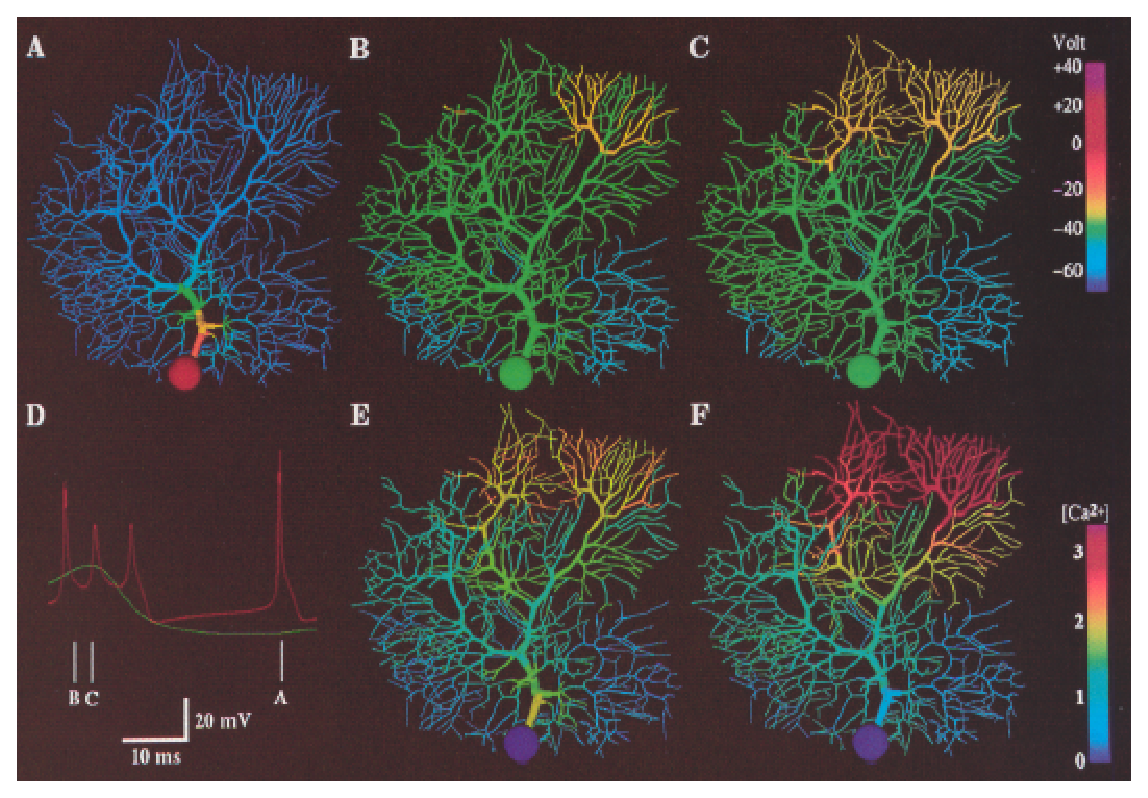
\includegraphics[scale=0.75]{figures/Fig.1.10.eps}
   \caption{False color representation of membrane potential and Ca$^{2+}$ concentration in the complete model during a 2.0\,nA current injection in the soma. {\it A}: Membrane potential distribution during a somatic action potential. {\it B}: Membrane potential distribution at the beginning of a dendritic spike. {\it C}: Membrane potential distribution 1.6\,ms later, when the dendritic spike had peaked. {\it D}: Somatic (red) and dendritic (green) recordings with the times when images A--C were taken indicated. {\it E}: Submembrane Ca$^{2+}$ concentration at same time as {\it B}. {\it F}: Submembrane Ca$^{2+}$ concentration at same time as {\it C}. Note the nonlinear voltage scale, which is expanded between -60 and -20\,mV.}
   \label{fig:DS1.10}
\end{figure}

\clearpage

\begin{figure}[h]
\centering
   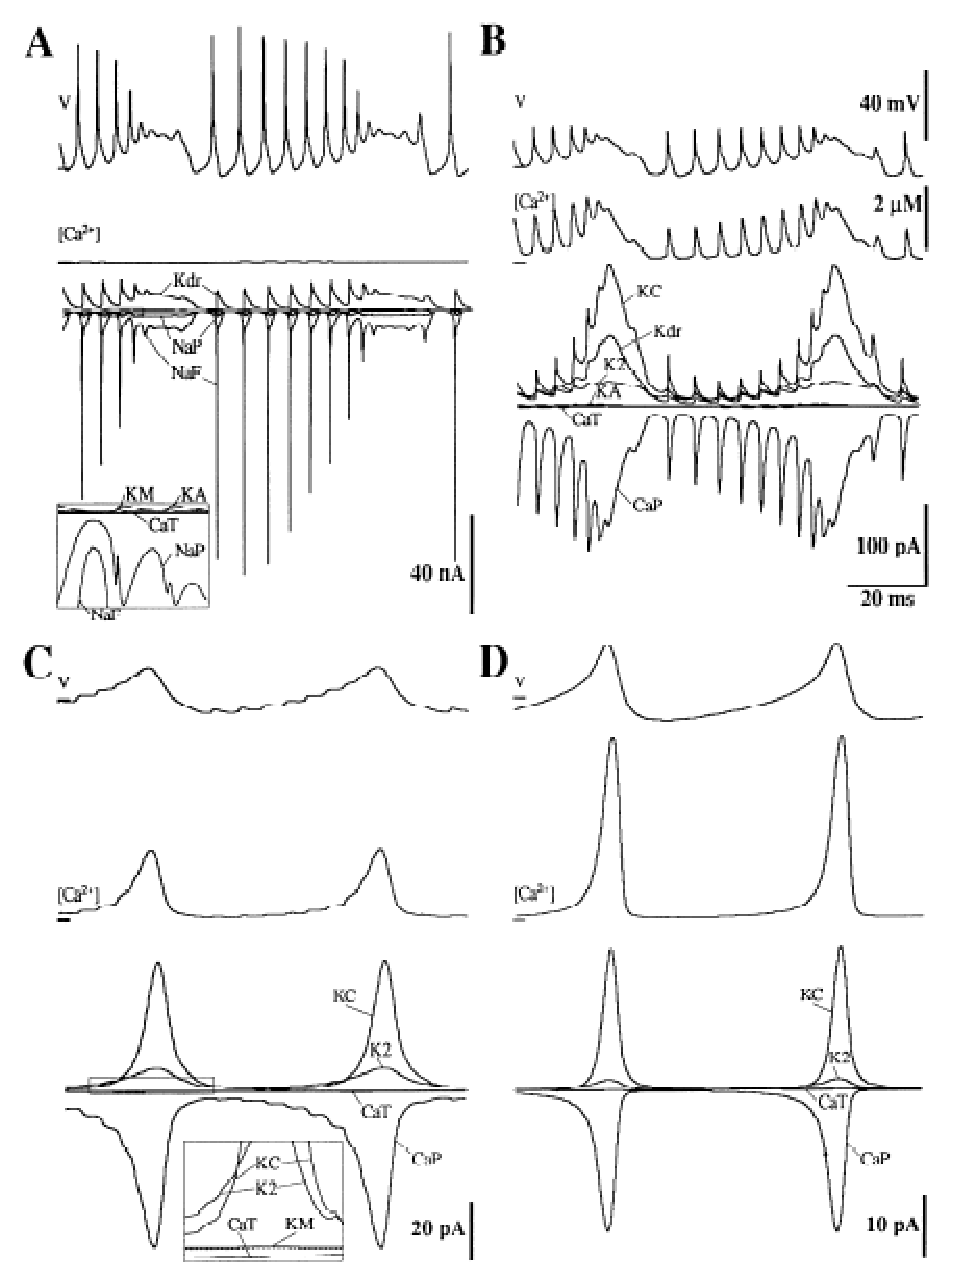
\includegraphics[scale=0.75]{figures/Fig.1.11.eps}
   \caption{Dynamic change in model variables during somatic and dendritic spikes. The same 100\,ms sequence is shown at 4 representative locations in the model during a 2.0\,nA current injection in the soma, 900\,ms after the start of the current injection (model PM9). {\it A}: Soma. {\it B}: Main dendrite. {\it C}: Smooth dendrite. {\it D}: Spiny dendrite. Each part of the figure shows the membrane potential (V, {\em top trace}), the Ca$^{2+}$ concentration ([Ca$^{2+}$], {\em middle trace}), and the amplitude of all ionic currents ({\em superimposed bottom traces}) in the compartment. {\it A} and {\it C}: Part of the current traces enlarged in a small box. The scale bars for voltage and concentration are identical in all sections. For the ionic currents each section is scaled differently (outward currents upward). Horizontal bar at {\em left} of V traces: -50\,mV membrane potential. Horizontal bar at {\em left} of [Ca$^{2+}$] traces: 0\,$\mu$M concentration. See Table 1 for abbreviations.}
   \label{fig:DS1.11}
\end{figure}

\clearpage

\begin{figure}[h]
\centering
   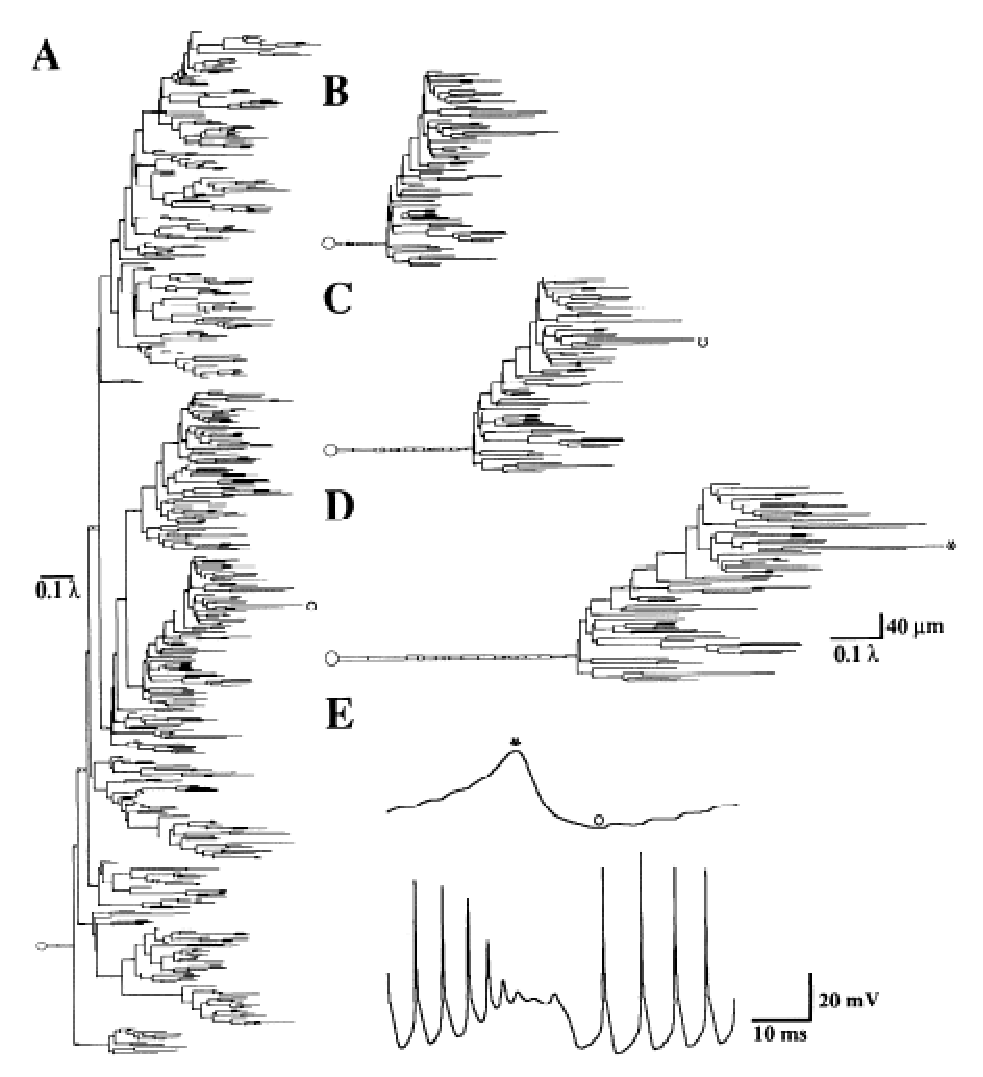
\includegraphics[scale=0.75]{figures/Fig.1.12.eps}
   \caption{Effect of voltage-dependent conductances on the electrotonic length of dendritic segments. {\it A} : Full Sholl diagram in units of electrotonic length of the cell with active conductances in the dendrites, during a pause in between action potentials. {\it B--D}: Enlargement of the Sholl diagram showing the same subset of branchlets (original location indicated by circle in {\it A}) under different conditions of the ionic channels. {\it B}: All passive membrane. {\it C}: Active membrane; the cell is in a quiet state in between action potentials (same as {\it A}). {\it D}: Active membrane at the peak of a dendritic spike. {\it E}: Recording of activity in a spiny dendrite ({\em top trace}, location marked on the Sholl diagrams) and soma ({\em bottom trace}). Dendrogram {\it D} was taken at the time indicated by the asterisk. Dendrogram {\it C} was taken at the time indicated by the circle. Simulation of 2.0\,nA current injection in the soma, model PM9.}
   \label{fig:DS1.12}
\end{figure}

\clearpage

\begin{figure}[h]
\centering
   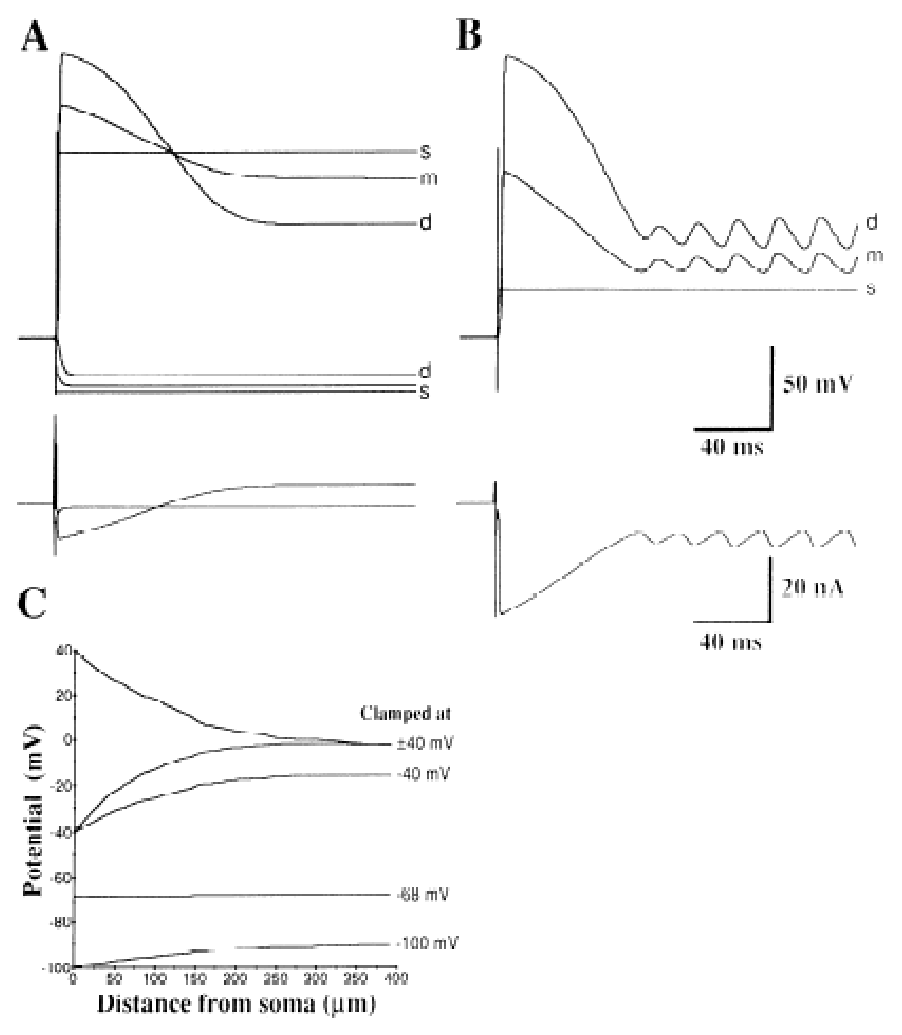
\includegraphics[scale=0.75]{figures/Fig.1.13.eps}
   \caption{Simulation of voltage-clamp steps. $A$: Model was clamped at resting potential (-68\,mV) and then stepped to -100 or +40 mV. Superimposed top traces: membrane potential in the soma (s), main dendrite ( m), and a distal spiny dendrite (d, marked with asterisk in Fig.\,1). Bottom trace: clamp current. $B$: as in $A$, but stepped to -40\,mV. $C$: membrane potential under steady-state voltage clamp vs. distance from the soma. Data from the same voltage-clamp steps as shown in $A$ and $B$. Data points are exclusively from compartments linking the soma with the distal spiny dendrite. Because the potential oscillated during steps to -40\,mV, 2 traces are shown for that voltage step (corresponding to the minimum and maximum voltage in the spiny dendrite). Simulation time step was 5\,$\mu$s.}
   \label{fig:DS1.13}
\end{figure}

\clearpage

\begin{figure}[h]
\centering
   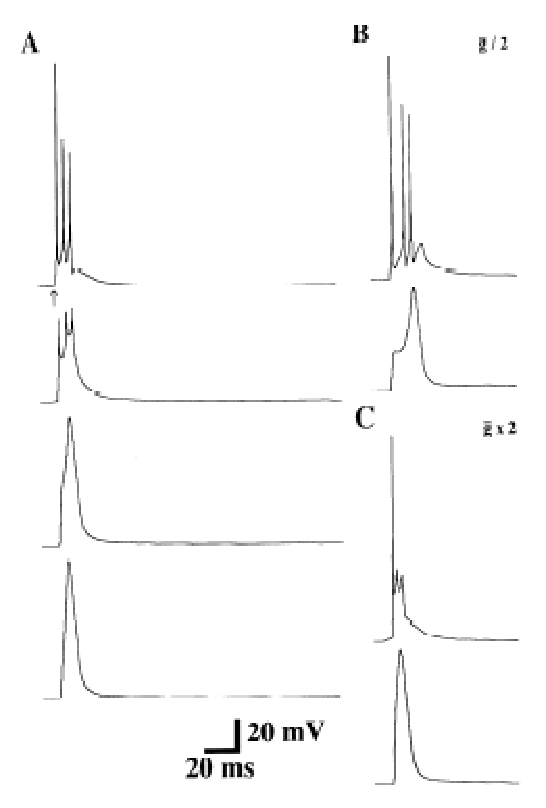
\includegraphics[scale=0.75]{figures/Fig.2.1.eps}
   \caption{Simulation of complex spike in slice. {\it A}: membrane potential before (-68\,mV) and during activation of the climbing fiber synapse as it would be recorded in (from {\em top} to {\em bottom}) the soma, the main dendrite, a smooth dendrite, and a spiny dendrite. See Fig. 1 in\,\cite{deschutter94:_purkin_i} for the specific locations of these recording sites in the model. {\it B}: Effect of changing maximum synaptic conductance ($\bar g$) of the climbing fiber synapse. Complex spike in the soma ({\em top}) and smooth dendrite with $\bar g$ at half of normal. {\it C}: Same as {\it B} with $\bar g$ at double normal.}
   \label{fig:DS2.1}
\end{figure}

\clearpage

\begin{figure}[h]
\centering
   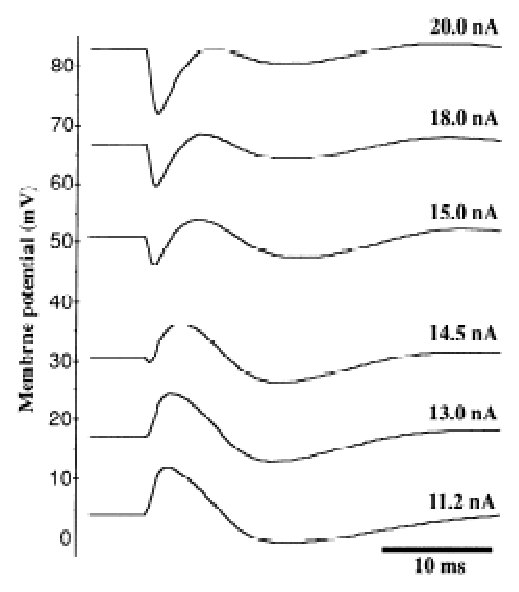
\includegraphics[scale=0.75]{figures/Fig.2.2.eps}
   \caption{Simulation of the dual reversal of the climbing fiber synapse. Membrane potential in the soma before and during a complex spike is shown under continuous current injections in the soma (current level indicated for each trace). See text for an explanation of the dual reversal.}
   \label{fig:DS2.2}
\end{figure}

\clearpage

\begin{figure}[h]
\centering
   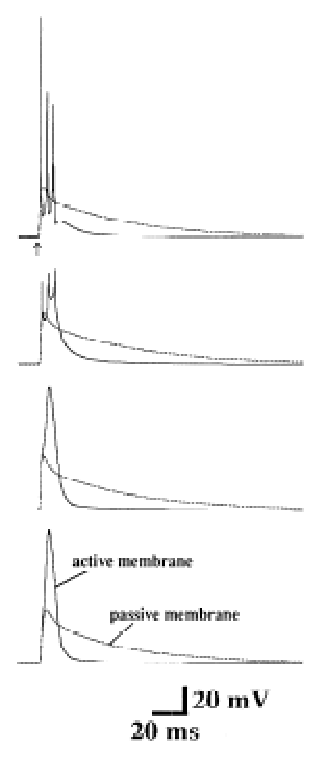
\includegraphics[scale=0.75]{figures/Fig.2.3.eps}
   \caption{Direct comparison of the response to climbing fiber activation in an active membrane and passive membrane model. The responses of the 2 models are superimposed. The active membrane responses are identical to those in Fig.\,1 and the same recording sites are used.}
   \label{fig:DS2.3}
\end{figure}

\clearpage

\begin{figure}[h]
\centering
   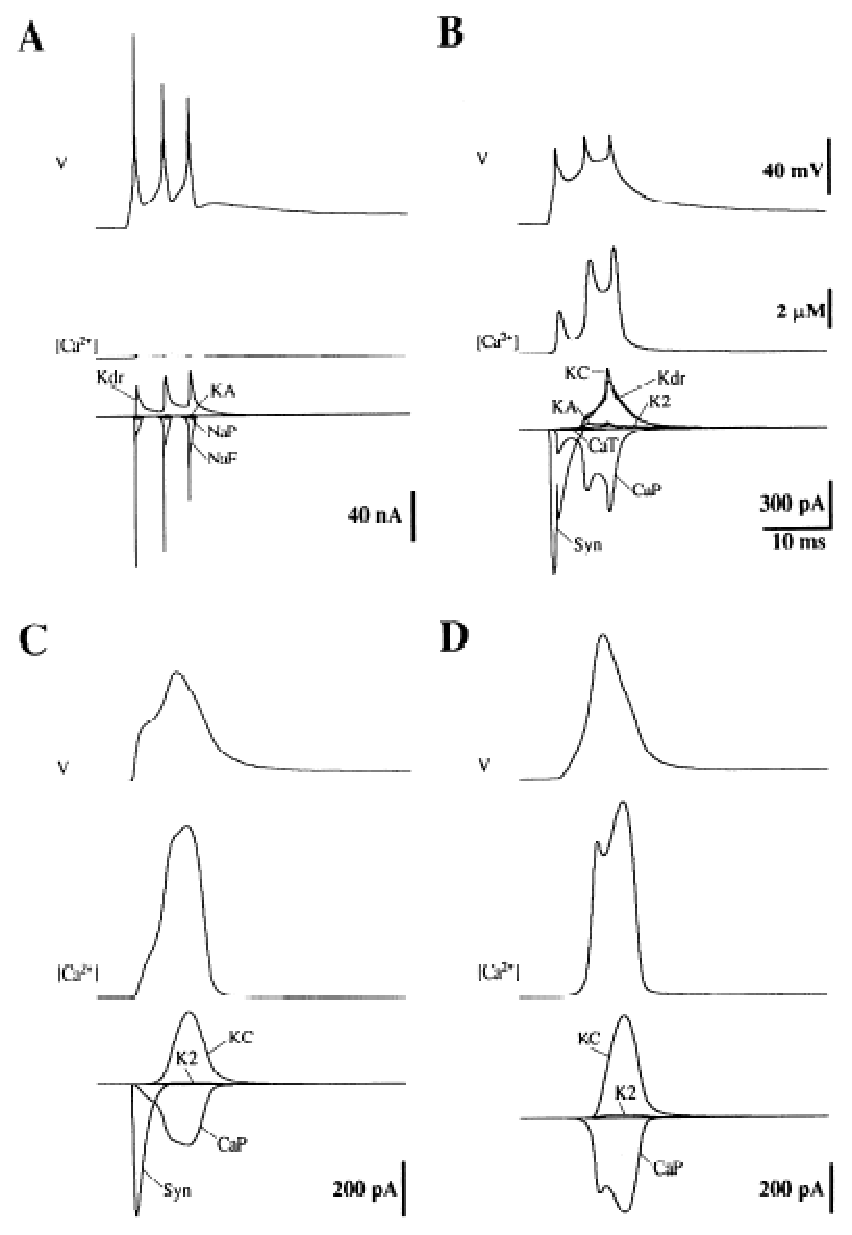
\includegraphics[scale=0.75]{figures/Fig.2.4.eps}
   \caption{Dynamic change in model variables during a complex spike at 4 representative locations in the model. {\it A}: Soma. {\it B}: Main dendrite. {\it C}: Smooth dendrite. {\it D}: Spiny dendrite. Each part of the figure shows the membrane potential ({\em top trace}), the Ca$^{2+}$ concentration ({\em middle trace}), and the amplitude of all ionic currents (superimposed {\em bottom traces}) in the compartment. In {\it B} and {\it C} the synaptic current (Syn) is also shown. The scale bars for voltage and concentration are identical in all sections; for the currents each section is scaled differently (outward currents upward). The model was at a stable resting membrane potential of -68\,mV before the complex spike. Kdr, delayed rectifier current; KA, A current; NaP, persistent sodium current; NaF, fast sodium current; KC, BK calcium-activated potassium current; K2, K2 calcium-activated potassium current; CaT, T calcium current; CaP, P calcium current.}
   \label{fig:DS2.4}
\end{figure}

\clearpage

\begin{figure}[h]
\centering
   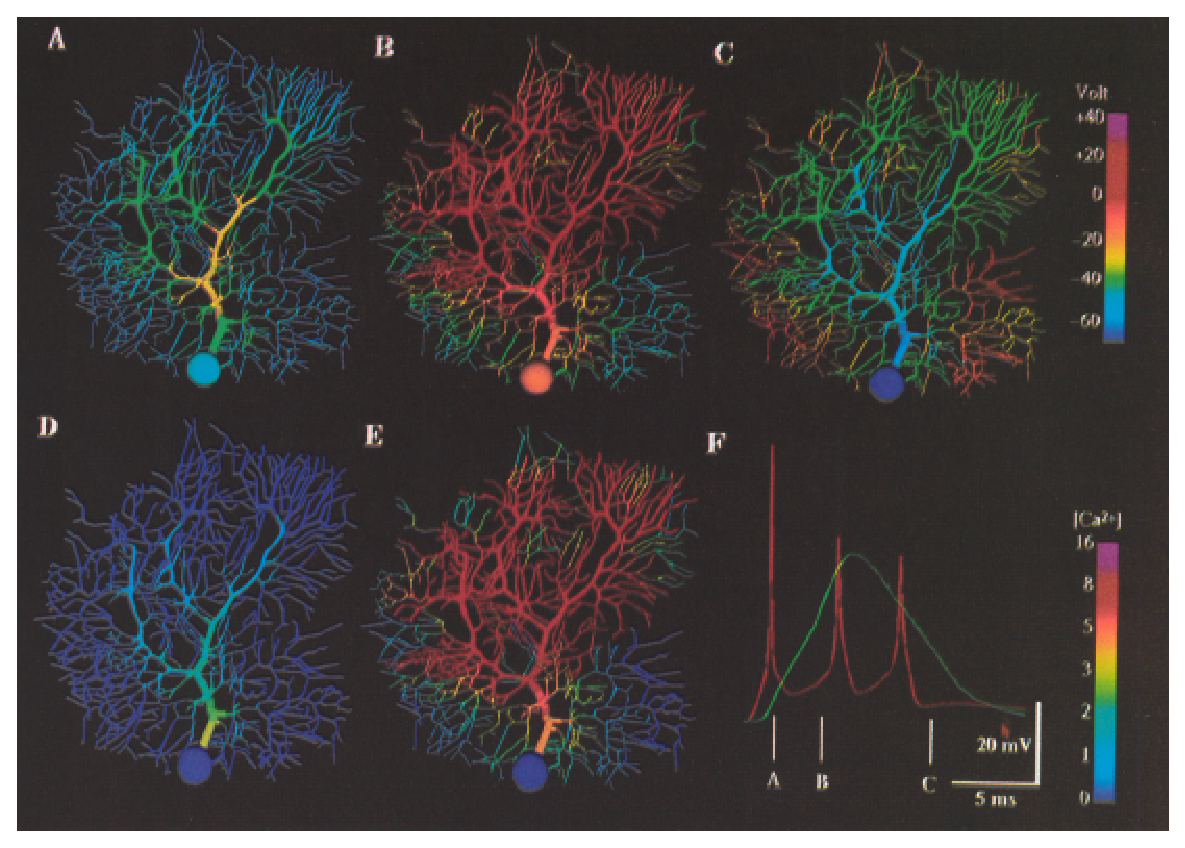
\includegraphics[scale=0.75]{figures/Fig.2.5.eps}
   \caption{False color representation of membrane potential and Ca$^{2+ }$ concentration in the complete model during complex spike. {\it A}: Membrane potential 1.4\,ms after beginning of complex spike. {\it B}: Membrane potential 4.0\,ms after beginning of complex spike. {\it C}: Membrane potential 10.0\,ms after beginning of complex spike (after the last somatic action potential). {\it D} and {\it E}: Submembrane Ca$^{2+}$ concentration at same times as {\it A} and {\it B}, respectively. {\it F}: Complex spike in the soma (red) and distal dendrite (green) with the time at which images {\it A--C} were taken indicated by white bars. Note the nonlinear [Ca$^{2+}$] scales.}
   \label{fig:DS2.5}
\end{figure}

\clearpage

\begin{figure}[h]
\centering
   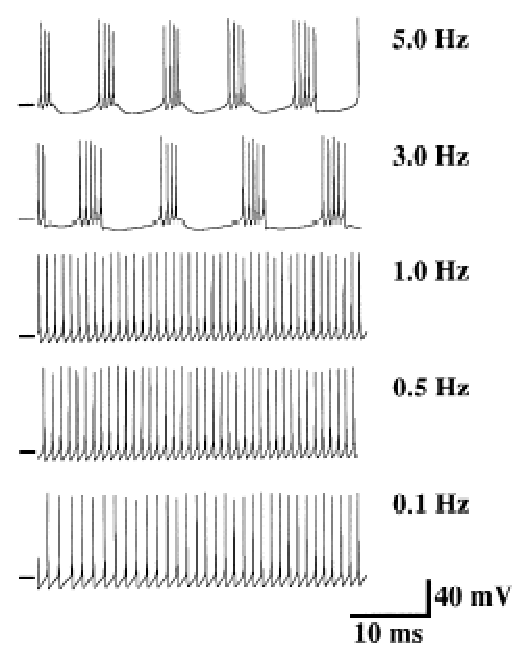
\includegraphics[scale=0.75]{figures/Fig.2.6.eps}
   \caption{Response of the Purkinje cell model to asynchronous excitation by 1,474 granule cell synapses firing at the average frequencies indicated. Membrane potential in the soma is shown. Bars at {\em left} of traces: -50\,mV membrane potential.}
   \label{fig:DS2.6}
\end{figure}

\clearpage

\begin{figure}[h]
\centering
   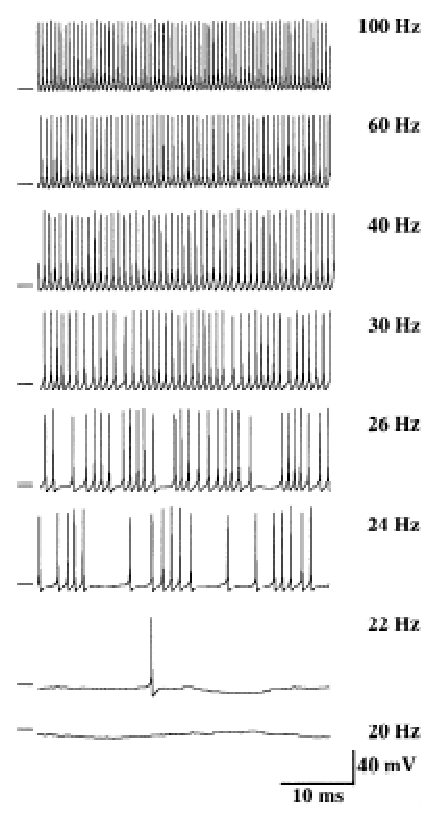
\includegraphics[scale=0.75]{figures/Fig.2.7.eps}
   \caption{Response of the Purkinje cell model to combined asynchronous excitation and inhibition. All the stellate cell synapses fired at an average rate of 1\,Hz; the 1,474 granule cell synapses fired at the average frequencies indicated. Membrane potential in the soma is shown. Bars at {\em left} of traces: -50\,mV membrane potential.}
   \label{fig:DS2.7}
\end{figure}

\clearpage

\begin{figure}[h]
\centering
   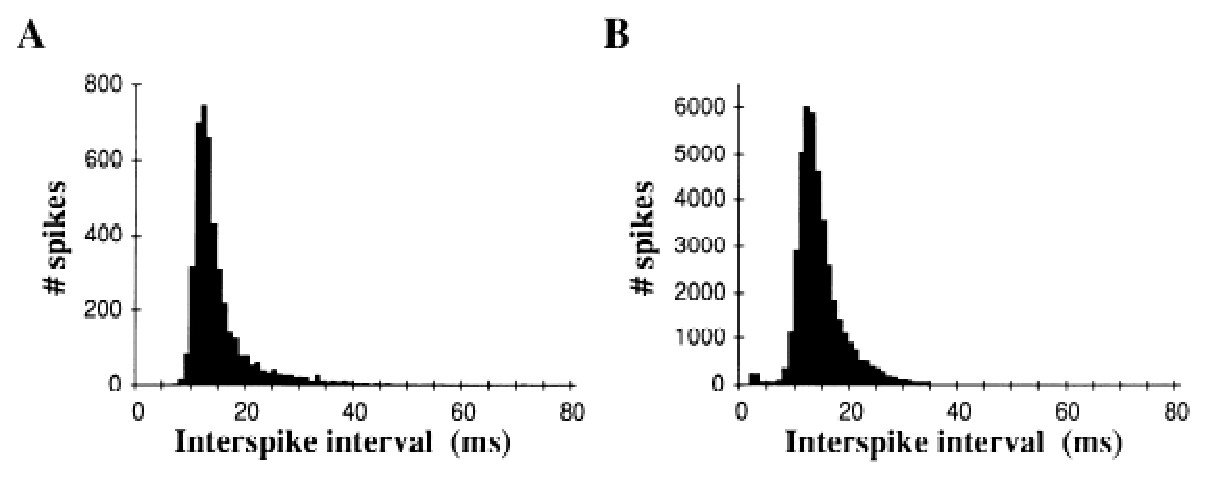
\includegraphics[scale=0.75]{figures/Fig.2.8.eps}
   \caption{Comparison of simulated and experimental interspike interval (ISI) distributions. {\it A}: ISI of simulated response to asynchronous excitation and inhibition. {\it B}: ISI constructed from in vivo extracellular Purkinje cell recording in crus IIa of the rat. Both ISIS have 1\,ms bin widths.}
   \label{fig:DS2.8}
\end{figure}

\clearpage

\begin{figure}[h]
\centering
   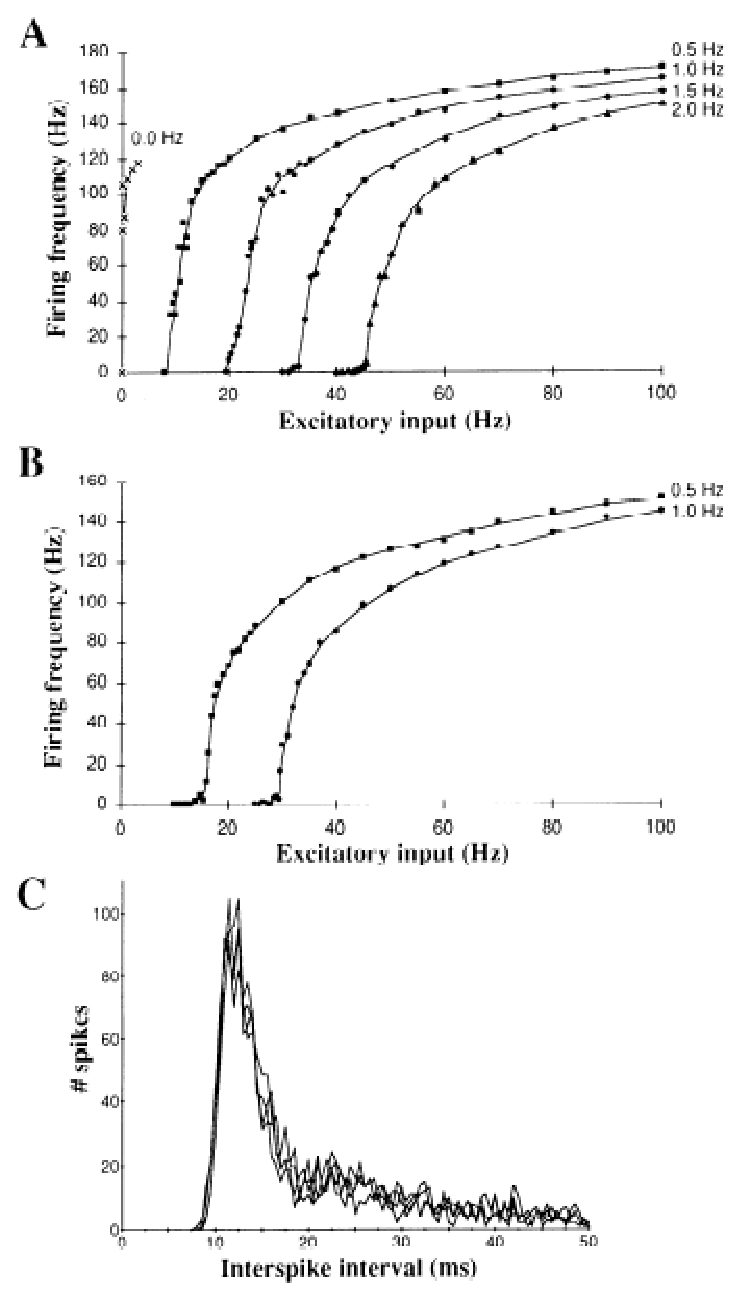
\includegraphics[scale=0.55]{figures/Fig.2.9.eps}
   \caption{Frequency response of the Purkinje cell model to different levels of excitation and inhibition. {\it A}: Frequency response curve for the PM9 model. The average firing frequency of the model is shown for different rates of asynchronous excitation and inhibition. The 5 curves correspond to the different frequencies of stellate cell inhibition indicated. Firing frequencies were computed over the interval of 1--2\,s simulated time for firing frequencies $>$50\,Hz and over the interval of 2--5\,s for lower frequencies. Note that these intervals were too short to completely average out the noise. {\it B}: frequency response curve for the PM10 model. {\it C}: interspike distributions of model PM9, firing at the same average frequency of 67\,Hz, caused by 4 different combinations of asynchronous excitatory and inhibitory input frequencies (10.4 and 0.5\,Hz, 23.5 and 1\,Hz, 37 and 1.5\,Hz, and 50 and 2\,Hz). The 4 ISIS are superimposed to facilitate comparison. Each IS1 based on 1,600 intervals. Bin width was 0.5\,ms.}
   \label{fig:DS2.9}
\end{figure}

\clearpage

\begin{figure}[h]
\centering
   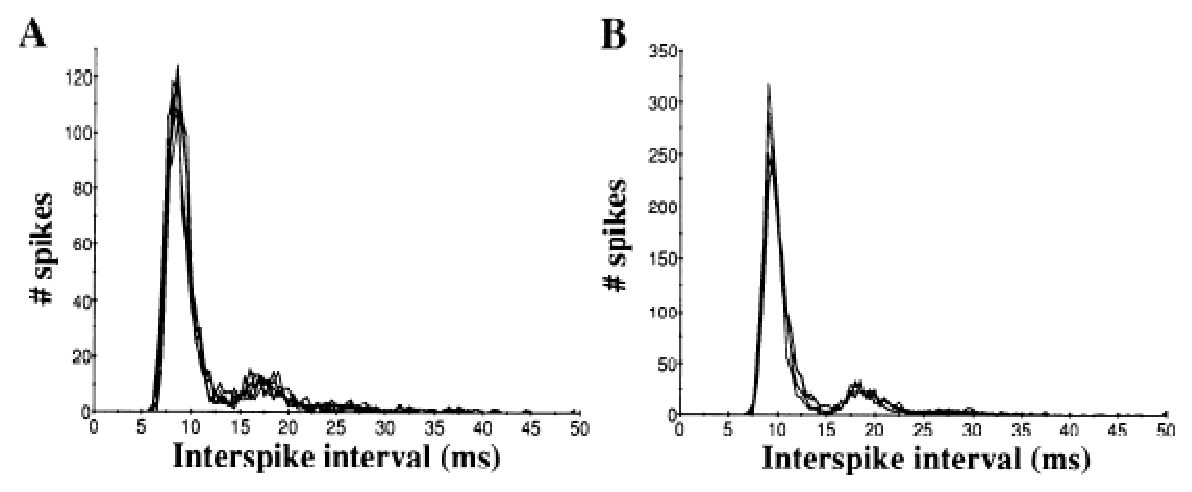
\includegraphics[scale=0.75]{figures/Fig.2.10.eps}
   \caption{Effect of scaling of number of inputs and of $\bar g$ 4 on simulated ISIS. {\it A}: ISI distributions for variable number of modeled spines. The ISIs have been superimposed to show similarity. Simulations were 500 spines firing asynchronously at 90\,Hz, 1,500 spines at 30\,Hz, 3,000 spines at 15\,Hz, 4,500 spines at 10\,Hz, 9,000 spines at 5\,Hz, and 14,000 spines at 3.21\,Hz. Each ISI is constructed of 800 events. Bin size is 1\,ms. {\it B}: Interspike distributions for 4 different maximum conductances of the granule cell synapse. Simulations were 1\,nS at 21\,Hz, 0.7\,nS at 30\,Hz, 0.35\,nS at 60\,Hz, and 0.1\,nS at 210\,Hz. Inhibition was always asynchronous at 1\,Hz. Each ISI is constructed of 1,600 events. Bin size is 1\,ms.}
   \label{fig:DS2.10}
\end{figure}

\clearpage

\begin{figure}[h]
\centering
   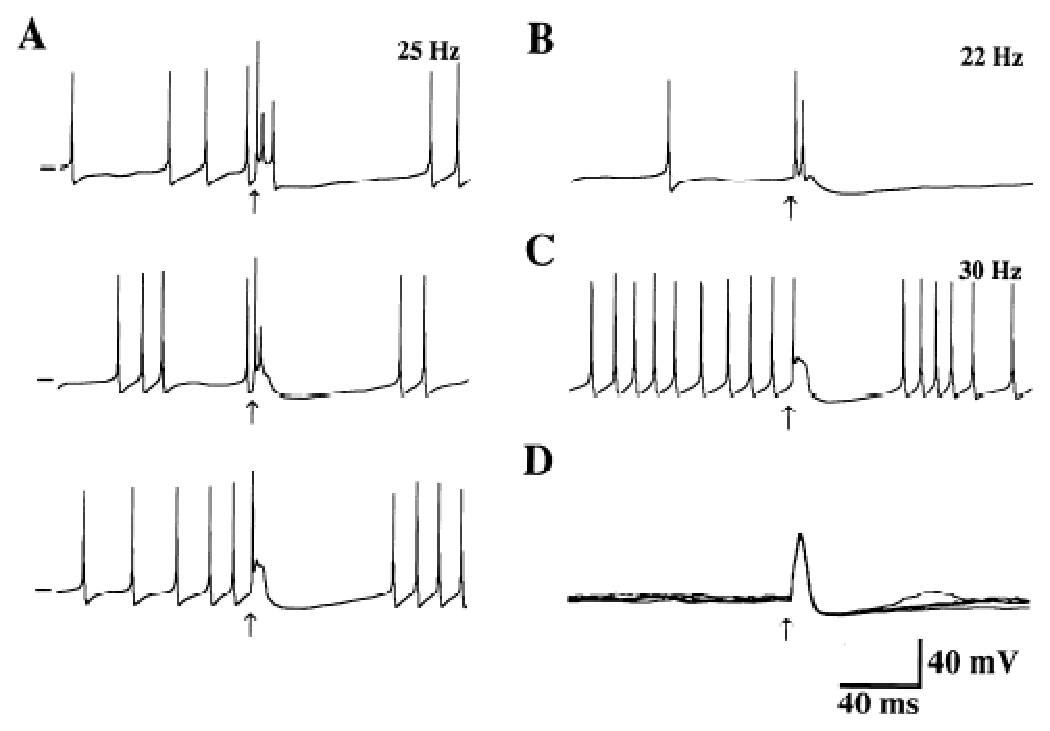
\includegraphics[scale=0.75]{figures/Fig.2.11.eps}
   \caption {Simulation of complex spikes in a Purkinje cell firing simple spikes. {\it A}: 3 different evoked complex spikes recorded in the soma during asynchronous excitation at 25\,Hz and inhibition at 1\,Hz. {\it B}: Complex spike recorded in the soma during asynchronous excitation at 22\,Hz. {\it C}: Complex spike in the soma during asynchronous excitation at 30\,Hz. {\it D}: Same complex spikes as in {\it A--C} in the smooth dendrite, traces superimposed.}
   \label{fig:DS2.11}
\end{figure}

\clearpage

\begin{figure}[h]
\centering
   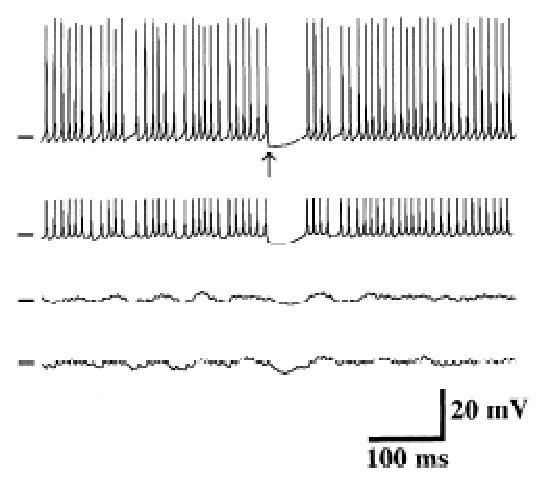
\includegraphics[scale=0.75]{figures/Fig.2.12.eps}
   \caption {Simulation of basket cell inhibition of a firing Purkinje cell neuron. At the time indicated, the equivalent of 20 basket cell synapses were activated. Membrane potential as it would be recorded in (from {\em top} to {\em bottom}) the soma, the main dendrite, a smooth dendrite, and a spiny
dendrite. The model was excited by asynchronous inputs at 30\,Hz and
inhibited at an asynchronous rate of 1\,Hz.}
   \label{fig:DS2.12}
\end{figure}

\bibliographystyle{plain}
\bibliography{../tex/bib/g3-refs}

\end{document}
